\documentclass[a4paper, 11pt, twoside]{article}

\usepackage{hyperref}
%\usepackage[ngerman]{babel}
\usepackage[english]{babel}
%\usepackage[latin1]{inputenc}
\usepackage[utf8]{inputenc}

\usepackage{graphicx,float,subfigure}
%\usepackage{pifont}
\usepackage{type1cm}
\usepackage{amssymb, amsthm, amsmath}
\usepackage{listings}
\usepackage{setspace} 

\usepackage{pgf}
\usepackage{url}
%\usepackage{graphicx}
%\usepackage{pifont}
%\usepackage{type1cm}


\usepackage{makeidx}
\makeindex

\setlength{\parindent}{0em}
\setlength{\oddsidemargin}{0.0cm}
\setlength{\evensidemargin}{0.0cm}
\setlength{\textheight}{23cm}
\setlength{\topmargin}{-0.5cm}
\setlength{\footskip}{1.5cm}
\setlength{\textwidth}{15.5cm}

\renewcommand*\familydefault{\sfdefault}

\newtheorem*{problem}{Problem}
\newcommand{\argmin}{\operatornamewithlimits{argmin}}

\lstnewenvironment{code}[1][]%
{\lstset{language=C++,
         basicstyle=\footnotesize\ttfamily,
         keywordstyle=\color{blue},
         tabsize=4,
         #1}
}{} 

\begin{document}
\thispagestyle{empty}

%\documentclass[a4paper]{article}

%\usepackage{pgf}
%\usepackage{graphicx}
%\usepackage{pifont}
%\usepackage{type1cm}

\setlength{\textwidth}{14cm}
\setlength{\oddsidemargin}{1cm}

%\begin{document}

\thispagestyle{empty}

%%%%%%%%%%%%%%%%%%%%%%%%%%%%%%%%%%%%%%%%
%%%%%%%%%%%%%%%%%%%%%%%%%%%%%%%%%%%%%%%%
%%%%%%%%%%%%%%%%%%%%%%%%%%%%%%%%%%%%%%%%

\newcount \Z
\Z=20

%%% logos %%%

%%% NUMHPC %%%
\newlength{\numhpclogox}
\setlength{\numhpclogox}{\paperwidth} % 20/210ths of the paperwidth
\divide\numhpclogox by 210
\multiply\numhpclogox by 100

\newlength{\numhpclogoy}
\setlength{\numhpclogoy}{\paperheight} % 270/297ths of the paperwidth
\divide \numhpclogoy by 297
\multiply \numhpclogoy by -235

\newlength{\numhpclogoheight}
\setlength{\numhpclogoheight}{\paperheight} % 270/297ths of the paperwidth
\divide\numhpclogoheight by 297
\multiply\numhpclogoheight by 20

%%% KIT %%%
\newlength{\kitlogox}
\setlength{\kitlogox}{\paperwidth} % 20/210ths of the paperwidth
\divide\kitlogox by 210
\multiply\kitlogox by 0

\newlength{\kitlogoy}
\setlength{\kitlogoy}{\paperheight} % 270/297ths of the paperwidth
\divide \kitlogoy by 297
\multiply \kitlogoy by -230

\newlength{\kitlogoheight}
\setlength{\kitlogoheight}{\paperheight} % 270/297ths of the paperwidth
\divide\kitlogoheight by 297
\multiply\kitlogoheight by 15


%%% EMCL %%%
\newlength{\emcllogox}
\setlength{\emcllogox}{\paperwidth} % 20/210ths of the paperwidth
\divide\emcllogox by 210
\multiply\emcllogox by 28

\newlength{\emcllogoy}
\setlength{\emcllogoy}{\paperheight} % 270/297ths of the paperwidth
\divide \emcllogoy by 297
\multiply \emcllogoy by -160

\newlength{\emcllogoheight}
\setlength{\emcllogoheight}{\paperheight} % 270/297ths of the paperwidth
\divide\emcllogoheight by 297
\multiply\emcllogoheight by 20

%%% HIFLOW %%%
\newlength{\hiflowlogox}
\setlength{\hiflowlogox}{\paperwidth} % 20/210ths of the paperwidth
\divide\hiflowlogox by 210
\multiply\hiflowlogox by 28

\newlength{\hiflowlogoy}
\setlength{\hiflowlogoy}{\paperheight} % 270/297ths of the paperwidth
\divide \hiflowlogoy by 297
\multiply \hiflowlogoy by -160

\newlength{\hiflowlogoheight}
\setlength{\hiflowlogoheight}{\paperheight} % 270/297ths of the paperwidth
\divide\hiflowlogoheight by 297
\multiply\hiflowlogoheight by 33

%%%%%%%%%%%%%%%%%%%%%%%%%%%%%%%%%%%%%%%%
%%%%%%%%%%%%%%%%%%%%%%%%%%%%%%%%%%%%%%%%
%%%%%%%%%%%%%%%%%%%%%%%%%%%%%%%%%%%%%%%%

%%% NUMHPC %%%
%%\pgftext[bottom, left, at={\pgfpointadd{\pgfpoint{0pt}{0pt}}{\pgfpoint{\numhpclogox}{\numhpclogoy}}}]{\includegraphics[totalheight=\numhpclogoheight]{numhpc}}

%%% KIT %%%
%%\pgftext[bottom, left, at={\pgfpointadd{\pgfpoint{0pt}{0pt}}{\pgfpoint{\kitlogox}{\kitlogoy}}}]{\includegraphics[totalheight=\kitlogoheight]{kitlogo}}

%%% EMCL %%%
\pgftext[bottom, left, at={\pgfpointadd{\pgfpoint{0pt}{0pt}}{\pgfpoint{\hiflowlogox}{\hiflowlogoy}}}]{
\includegraphics[totalheight=\hiflowlogoheight]{HF3_color}}

%%% horizontal lines %%%
\pgfline{\pgfxy(-1pt,0.1pt)}{\pgfxy(15pt,0.1pt)}
\pgfline{\pgfxy(-1pt,-21.4pt)}{\pgfxy(15pt,-21.4pt)}
%%\pgfline{\pgfxy(-1pt,-22.4pt)}{\pgfxy(15pt,-22.4pt)}

%%% EMCL text %%%
\pgftext[bottom, left, at={\pgfpointadd{\pgfpoint{0pt}{0pt}}{\pgfpoint{0cm}{1cm}}}]{{\LARGE{{\bf Tutorial}}}}

%%% EMCL web %%%
\pgftext[bottom, left, at={\pgfpointadd{\pgfpoint{0pt}{0pt}}{\pgfpoint{10.5cm}{-21.7cm}}}]{{\fontsize{13}{10}\selectfont{} http://www.hiflow3.org/}}

\hspace{2cm}
\begin{picture}(0,0)(-250,-25)

\includegraphics[scale=.22]{emcl.pdf} 
\end{picture}

%%% author %%%
\pgftext[bottom, left, at={\pgfpointadd{\pgfpoint{0pt}{0pt}}{\pgfpoint{0cm}{-4cm}}}]{{
\begin{parbox}{13cm}{
\begin{center}\fontsize{12}{30}\selectfont{} J. Kr\"amer, A. Sommer, A. Helfrich-Schkarbanenko
\end{center}}
\end{parbox}}}

%%% title %%%
\pgftext[bottom, left, at={\pgfpointadd{\pgfpoint{0pt}{0pt}}{\pgfpoint{0cm}{-7.5cm}}}]{{
\begin{parbox}{13cm}{
%%\begin{center}\fontsize{18}{30}\selectfont{} \bf Using HiFlow$^3$ for solving the
\begin{center}\fontsize{22}{30}\selectfont{} \bf Direct and Inverse Problem\\ in Electrostatics
\end{center}}
\end{parbox}}}

%%% date %%%
\pgftext[bottom, left, at={\pgfpointadd{\pgfpoint{0pt}{0pt}}{\pgfpoint{0cm}{-16.4cm}}}]{{
\begin{parbox}{13cm}{
\begin{center}\fontsize{12}{24}\selectfont{} 
\vspace{5cm}
\textit{modified on \today}\\ 
\vspace{6.5cm}
\hspace{6cm}\textit{Version 1.4}
\end{center}}
\end{parbox}}}

%fhfh \hfill sjdh

%\end{document}


%\newpage
%\null\newpage

\newcommand{\dd}{\mathrm{d}}
\newtheorem{remark}{Remark}[section]
\thispagestyle{empty}
\tableofcontents

\newpage
\pagestyle{plain}
\framebox[15.5cm]{\parbox[c][2.3cm]{14.0cm}{
{\fontsize{19}{30}\selectfont{} \bf{Applying HiFlow$^3$ for solving direct and\\inverse problem in electrostatics}
}}}
\vspace{0.5cm}

\section{Introduction}

HiFlow$^3$ is a multi-purpose finite element software providing powerful tools for efficient and accurate solution of a wide range of problems modeled by partial differential equations (PDEs). Based on object-oriented concepts and the full capabilities of C++ the HiFlow$^3$ project follows a modular and generic approach for building efficient parallel numerical solvers. It provides highly capable modules dealing with the mesh setup, finite element spaces, degrees of freedom, linear algebra routines, numerical solvers, and output data for visualization. Parallelism - as the basis for high performance simulations on modern computing systems - is introduced on two levels: coarse-grained parallelism by means of distributed grids and distributed data structures, and fine-grained parallelism by means of platform-optimized linear algebra back-ends.


\subsection{How to Use the Tutorial?}
You find the example code (direct\_inverse\_tutorial.cc, direct\_inverse\_tutorial.h) and a parameter file for the first numerical example (direct\_inverse\_tutorial.xml)  
  in the folder  \\ 
  \verb'/hiflow/examples/direct_inverse'. The geometry data (*.inp, *.vtu) is stored in the folder \verb'/hiflow/examples/data'.

\subsubsection{Using HiFlow$^3$ as a Developer}\label{sectiondeveloper}
First build and compile HiFlow$^3$. Go to the directory \verb'/build/example/direct\_inverse', where the binary \textbf{direct\_inverse\_tutorial} is stored. Type \textbf{./direct\_inverse\_tutorial}, to execute the program in sequential mode. To execute in parallel mode \index{program!executing in parallel} with four processes, type \textbf{mpirun -np 4 ./direct\_inverse\_tutorial}. In both cases, you need to make sure that the default parameterfile direct\_inverse\_tutorial.xml is stored in the same directory as the binary, and that the geometry data specified in the parameter file is stored in \verb'/hiflow/examples/data'. Alternatively, you can specify the path of your own xml-file with the name of your xml-file (first) and the path of your geometry data (second) in the comment line, i.e. \textbf{./direct\_inverse\_tutorial} \verb'/"path_to_parameterfile"/"name_of_parameterfile".xml' \verb'/"path_to_geometry_data"/'.

\section{Mathematical Setup}
%
In this tutorial we study an elliptic boundary value problem with Robin boundary condition\index{boundary condition!Robin} arising in electrostatics  in a bounded Lipschitz domain $\Omega\subset\mathbb{R}^3$. We aim to reconstruct the current source $f:\overline{\Omega}\to\mathbb{R}$ with $supp(f)\subset\Omega$ on the basis of some local electric potential data $u_d$, assuming the electrical conductivity $\sigma:\overline{\Omega}\to\mathbb{R}_{\ge 0}$ is known. By local data we mean the restriction $u_d:=u|_{\Gamma}$ of $u:\overline{\Omega}\to\mathbb{R}$ to a subdomain (path) $\Gamma\subset\Omega$ with $supp(f)\;\cap\;\Gamma=\emptyset$. To set up this so called "inverse problem" we firstly have to focus on the direct problem.

\subsection{Direct Problem}
Our aim is to find $u\in C^2(\Omega)\cap C^1(\overline{\Omega})$ that satisfies
%
\begin{eqnarray}\label{eq:strongproblem}
\begin{array}{rcll}
	-\nabla\cdot(\sigma\nabla u) &=& f, & \text{ in }\Omega,\\
	\frac{\partial u}{\partial\nu}+gu &=& 0, & \text{ on }\partial\Omega,
\end{array}
\end{eqnarray}
%
where $f \in C(\Omega)$ and $\sigma\in C^1(\Omega)\cap C(\overline \Omega)$ are given. The function $g\in L^\infty_{>0}(\partial\Omega)$ describes the reciprocal distance between the boundary and the center of $supp(f)$. The Robin boundary condition on the artificial boundary $\partial\Omega$ forces the electric potential $u$ to decrease reciprocally proportional to the distance between $\partial\Omega$ and the source. Doing so we imitate $\Omega$ to be unbounded, i.e. we minimize the influence of the artificial introduced boundary $\partial\Omega$ on the solution $u$, cf. Figure \ref{fig:skizze}.\\

\begin{figure}[ht]
\centering 
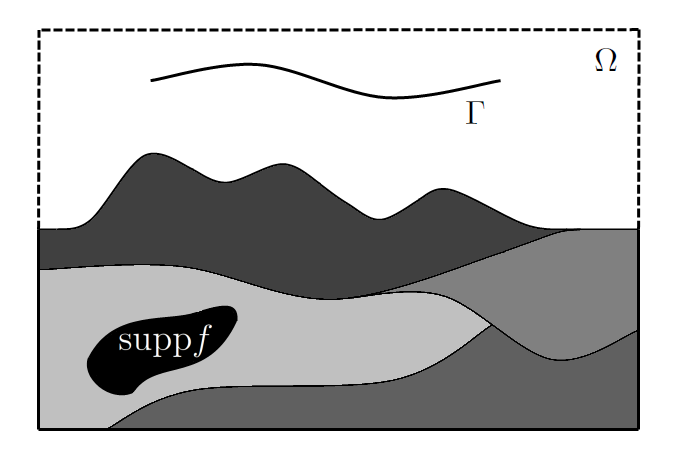
\includegraphics[width=6cm]{skizze.png}
\caption{Scenario for the problem to investigate.}
\label{fig:skizze}
\end{figure}
%
Referring to the Poisson Tutorial, finding classical solutions of \eqref{eq:strongproblem} is difficult. To produce relief we have to reformulate this problem to the corresponding weak formulation, which requires weaker assumptions on the regularity of $u$, $f$ and $\sigma$.

\subsubsection{Weak Formulation}\label{sectionWeak_formulation}
We consider the Hilbert space $L^2(\Omega)$, where the evolution equation and the boundary condition in \eqref{eq:strongproblem} can be combined to one integral equation. Let $u$, $f$ and $\sigma$ be as in the strong formulation \eqref{eq:strongproblem}. To set up the weak formulation we multiply both sides of conductivity equation in \eqref{eq:strongproblem} with a test function $\varphi\in C^\infty(\Omega)$ and integrate over $\Omega$:
%
\begin{equation*}
	\int_\Omega-\nabla\cdot(\sigma\nabla u)\,\varphi\,\dd x=\int_\Omega f\,\varphi\,\dd x.
\end{equation*}
%
Since $\Omega$ has Lipschitz boundary $\partial\Omega$, Green's first identity and the Gaussian integral theorem can be applied
%
\begin{equation}\label{eq:varformulation}
	\int_\Omega\sigma\nabla u\cdot\nabla\varphi\,\dd x-\int_{\partial\Omega}\sigma(\nabla u\cdot n)\varphi\,\dd o=\int_\Omega f\varphi\,\dd x,
\end{equation}
%
where $n$ is the (outer) normal vector on $\partial \Omega$. Since our boundary value problem contains natural boundary conditions, the Robin boundary condition $(\nabla u\cdot n)=-gu$ on $\partial\Omega$ can be integrated in \eqref{eq:varformulation}:
%
\begin{equation}\label{eq:varformulation2}
	\int_\Omega\sigma\nabla u\cdot\nabla\varphi\,\dd x+\int_{\partial\Omega}\sigma\,g\,u\,\varphi\,\dd o=\int_\Omega f\varphi\,\dd x \qquad\forall\varphi\in C^\infty(\Omega).
\end{equation}
%
Introducing the Sobolev space $H^2(\Omega):=\{u\in L^2(\Omega):D^{\alpha}u\in L^2(\Omega)\quad\forall\,|\alpha|\le 2\}$ for the solution $u$, see Braess \cite{bib:bra03}, completes the derivation of the weak formulation. Because $C^\infty(\Omega)$ is dense in $H^2(\Omega)$ it is convenient to choose $\varphi\in H^2(\Omega)$, which yields
%
\begin{equation}\label{eq:varformulation3}
	\int_\Omega\sigma\nabla u\cdot\nabla\varphi\,\dd x+\int_{\partial\Omega}\sigma\,g\,u\,\varphi\,\dd o=\int_\Omega f\varphi\,\dd x \qquad \forall \varphi\in H^2(\Omega).
\end{equation}
%
Consequently, we need the following weaker assumptions: $f\in L^2(\Omega)$, with $supp(f)\subset\Omega$ and $\sigma\in L^2(\Omega)$ with $0<1/C<\sigma(x)<C$ for all $x\in\Omega$ and $C>0$. Now our aim is to find the so called weak solution $u\in H^2(\Omega)$ that solves equation \eqref{eq:varformulation3}.\\
Actually, the Sobolev space $H^1(\Omega)$ is sufficient for the weak formulation, see Sommer \cite{bib:som12}. But with respect to the inverse problem in Section \ref{sec:reginvpro} we will see that the regularity $u\in H^2(\Omega)$ is necessary, because of the measurement methodology. This does not cause any difficulties, because applying the regularity theorem \cite[Thm.\;8.13,\;8.14]{bib:sal08} yields $u\in H^2(\Omega)$ if $f\in L^2(\Omega)$ and $\partial\Omega$ is sufficient smooth, i.e. $C^2$ bound.\\
The weak formulation can be rewritten in brief formulation as follows: Find $u\in H^2(\Omega)$ that fulfills the integral equation
%
\begin{equation}\label{eq:weakformulationsobolev}
	a(u,\varphi)\ =\ l(\varphi) \quad \forall \varphi \in H^2(\Omega),
\end{equation}
%
where the bilinear form $a:H^2(\Omega)\times H^2(\Omega)\rightarrow\mathbb{R}$ defined by
\begin{equation*}
	a(u,\varphi)=\int_\Omega\sigma\nabla u\cdot\nabla\varphi\,\dd x+\int_{\partial\Omega}\sigma\,g\,u\,\varphi\,\dd o  
\end{equation*}
is continuous and elliptic. The linear form $l:L^2(\Omega)\rightarrow\mathbb{R}$ 
\begin{equation*}
	l(\varphi) = \int_\Omega f\, \varphi\, \dd x
\end{equation*}
is continuous, see Braess \cite[Def.\;2.4]{bib:bra03}. Because of these properties the direct problem satisfies the Lax-Milgram Lemma \cite{bib:gil01} and is therefore uniquely solvable.\\
Due to C\'{e}as lemma \cite{bib:bra03} we can discretize the problem in the sense of Galerkin without disturbing the unique solvability. That means, we can solve the weak formulation \eqref{eq:weakformulationsobolev} uniquely in a finite dimensional subspace
%
\[H^2_h(\Omega)\subset H^2(\Omega)\]
%
for an example via FEM. A detailed proof is given by Sommer \cite{bib:som12}. So we apply HiFlow$^3$ to find $u_h \in H^2_h(\Omega)$, which approximates the weak solution $u\in H^2(\Omega)$.\\

In respect of the inverse problem this weak formulation of boundary value problem \eqref{eq:strongproblem} can be transferred to a brief operator equation
\begin{equation}\label{eq:Af=u}
 \Lambda[f]\ =\ u,
\end{equation}
where the bounded, linear forward operator denoted by 
\begin{equation*}
	\Lambda:\,\left\{\begin{array}{ccc}
	L^2(\Omega) &\to &H^2(\Omega),\\
	f &\mapsto &u,
\end{array}\right.
\end{equation*}
maps given current density $f$ onto electric potential $u$. Especially, $\Lambda$ represents the governing physics. 
%
%============================================================================================================
% Numerical Implementation of the Inverse Problem
%============================================================================================================
%
\subsubsection{Numerical Implementation}
%
In the following we emphasize that the numerical linear operators are matrices and the discrete functions were represented by vectors. Recalling by C\'{e}a Lemma \cite{bib:bra03} we can solve the direct problem in a finite dimensional subspace $H^2_h(\Omega)\subset H^2(\Omega)$ without loosing the uniqueness of the solution. Thus, the weak formulation \eqref{eq:weakformulationsobolev} can be presented in matrix notation
%
\begin{equation}\label{eq:finiteelement}
	\boldsymbol{A}\boldsymbol{u}=\boldsymbol{l}\quad\text{for all}\;\varphi_k\in H^2_h(\Omega),
\end{equation}
%
where $\boldsymbol{A}\in\mathbb{R}^{n\times n}$ is the stiffness matrix, cf. HiFlow$^3$ Source Code in Listings \ref{sc:stiffness}, \ref{sc:robin}, \ref{sc:sigma} and \ref{sc:g}, with elements
%
\begin{equation*}
	\boldsymbol{A}_{i,j}=\int_{\Omega}\sigma\nabla\varphi_i\cdot\nabla\varphi_j\,dx
	+\int_{\partial\Omega}\sigma\,g\,\varphi_i\,\varphi_j\,ds,
\end{equation*}
%
$\boldsymbol{l}\in\mathbb{R}^n$ the right hand side, cf. Listing \ref{sc:rhs}, with entries
%
\begin{equation*}
	\boldsymbol{l}_{i}=\int_{\Omega}f\,\varphi_i\,dx,
\end{equation*}
%
$\boldsymbol{u}\in\mathbb{R}^n$ is the nodal electric potential vector and $f:L^2(\Omega)\to\mathbb{R}$ is the current source density function. The basis functions $\{\varphi_i\}^n_{i=1}$ are in the finite dimensional subspace $H^2_h(\Omega)$ of the Sobolev space $H^2(\Omega)$. The number of degrees of freedom of the model is denoted by $n$. Solving the direct problem means solving equation \eqref{eq:finiteelement}. But to set up the discrete forward operator $\boldsymbol{\Lambda}$ it is useful to represent the source function $f$ by its nodal source vector $\boldsymbol{f}\in\mathbb{R}^n$, cf. Listing \ref{sc:f}, so that \eqref{eq:finiteelement} can be extended to
%
\begin{equation}\label{eq:finiteelement2}
	\boldsymbol{A}\boldsymbol{u}=\boldsymbol{M}\boldsymbol{f}\quad\text{for all}\;\varphi_k\in H^2_h(\Omega),
\end{equation}
%
where $\boldsymbol{M}\in\mathbb{R}^{n\times n}$ is the mass matrix with entries
%
\begin{equation}\label{eq:massmatrix}
	\boldsymbol{M}_{i,j}=\int_{\Omega}\varphi_i\,\varphi_j\,dx.
\end{equation}
%
Based on equation \eqref{eq:finiteelement2} we find the discrete forward operator
%
\begin{equation*}
	\boldsymbol{\Lambda}=\boldsymbol{A}^{-1}\boldsymbol{M},
\end{equation*}
%
cf. Listing \ref{sc:lambda}. Since the stiffness matrix $\boldsymbol{A}$ is symmetric and positive definite, see Sommer \cite{bib:som12}, it is invertible. It can be shown that the mass matrix $\boldsymbol{M}$ is symmetric, positive definite, too. Hence, the product $\boldsymbol{\Lambda}$ is invertible, but in general not positive definite and non-symmetric.\\

%-----------------------------------------------------------------------------------
% alte Version - eventuell bei Parallelisierung wieder notwendig!
%-----------------------------------------------------------------------------------
%Note that the inverse $\boldsymbol{A}^{-1}$ has to satisfy the equation $\boldsymbol{AA}^{-1}=\boldsymbol{I}$. Considering this equation column by column leads to computation of the $i$-th column $\boldsymbol{a}^{-1}_i$ of the inverse $\boldsymbol{A}^{-1}$ by
%\begin{equation*}
%	\boldsymbol{Aa}^{-1}_i=\boldsymbol{e}_i\quad\text{for}\;i=1,\ldots,n,
%\end{equation*}
%where $\boldsymbol{e}_i$ is the unit vector with one in $i$-th row.\\
%-----------------------------------------------------------------------------------

In the actual HiFlow$^3$ Source Code the inverse operators are being avoided, since the full invertation of a $n \times n$-matrix is very expensive for large $n$. Therefore $\boldsymbol{\Lambda}$ are computed by a series of linear systems of equations
\[
\boldsymbol{A} \boldsymbol{\Lambda}_i = \boldsymbol{M}_i,
\]
for all $i=1,...,n$, cf. Listing \ref{sc:lambda}, where $\boldsymbol{\Lambda}_i$ and $\boldsymbol{M}_i$ are the $i^{th}$ column of $\boldsymbol{\Lambda}$ and $\boldsymbol{M}$, respectively.

%
%============================================================================================================
% Inverse Problem
%============================================================================================================
%
%\newpage
\subsection{Inverse Problem}\label{sec:invpro}

In this section we present an approach how to reconstruct $f$ from some local data $u_d$.\\

In practice it is impossible to measure $u$ in the whole domain $\Omega$. Thus, we have to introduce a subdomain $\Gamma\subset\Omega$ with $supp(f)\;\cap\;\Gamma=\emptyset$, on which measurements are available. To restrict $u$ to the local synthetic data $u_d:=u|_\Gamma$ we define an operator
%
\begin{equation}\label{eq:restrictionoperator}
	T:\,\left\{\begin{array}{ccc}
	H^2(\Omega) &\to &L^2(\Gamma),\\
	u &\mapsto &u_d:=u|_{\Gamma},
\end{array}\right.
\end{equation}
%
which is necessary to generate local synthetic data
%
\begin{equation*}
	u_d = Tu = T\Lambda[f].
\end{equation*}
%
Note that the restriction to $u_d\in L^2(\Omega)$ is only possible if $u\in H^2(\Omega)$ is assumed, as shown by Sommer \cite{bib:som12}. This is the reason why in the weak formulation the regularity $u\in H^2(\Omega)$ was chosen. Combination of $\Lambda$ with $T$ leads to the following ill-posed inverse problem:
%============================================================================================================
\begin{problem}
For given local measurements $u_d\in L^2(\Gamma)$ find $f\in L^2(\Omega)$ such that
\begin{equation}\label{pro:invpro}
	T\Lambda[f]=u_d
\end{equation}
holds.
\end{problem}
%============================================================================================================
The essential point here is the usage of the restriction operator $T$. It restricts an electric potential $u$ to local synthetic data $u_d$. The consequence is that $T\Lambda$ is non-injective. For example one small dipole source below ground level generates the same data $u_d$ in the air as one big source in greater depth, see Sommer \cite[Chap.\;4.2.1]{bib:som12}. Because of that non-injectivty of $T\Lambda$ the inverse problem \eqref{pro:invpro} is ill-posed in sense of Hadamard \cite{bib:had15}. In the discrete case the Matrix $\boldsymbol{T\Lambda}$ is strongly under-determined and thus singular. Hence, it can not be inverted and a regularizing technique should be applied.
%
%============================================================================================================
% Regularized Inverse Problem
%============================================================================================================
%
\subsubsection{Regularized Inverse Problem}\label{sec:reginvpro}
%
We know that a solution of the inverse problem \eqref{pro:invpro} exists, but it is non-unique. Hence the inverse problem \eqref{pro:invpro} is ill-posed. However, applying the idea of Tikhonov \cite{bib:tik63}, which is explained in next paragraph, we can enforce this uniqueness.\\

The concept of Tikhonov regularization is the following: If no true solution can be computed, we modify the problem in such way that the corresponding new solution, which is called "pseudo-solution", is unique and in relation to the true solution. In detail, the Tikhonov regularization consists of perturbation of an operator via spectral shift to enforce the uniqueness of a pseudo-solution. For further information we refer to Kirsch \cite{bib:kir96}, Rieder \cite{bib:rie03}. Doing so we obtain the regularized inverse problem for local measurements:
%============================================================================================================
\begin{problem}
Let $u_d\in L^2(\Gamma)$ be local synthetic data on $\Gamma\subset\Omega$. Find $f\in L^2(\Omega)$ by solving the minimization problem
%
\begin{equation}\label{eq:reginvpro}
  f_{L,\alpha}=
  \argmin_{f\in L^2(\Omega)}\big\{\tfrac{1}{2}\|T\Lambda[f]-u_d\|^2_{L^2(\Gamma)}
  +\tfrac{\alpha}{2}\|f\|^2_{L^2(\Omega)}\big\},
\end{equation}
%
%\begin{equation}\label{eq:reginvpro}
%  f_{L,\alpha}=
%  arg \min_{f\in L^2(\Omega)}\big\{\tfrac{1}{2}\|(T\Lambda)\,f-u_d\|^2_{L^2(\Gamma)}
%  +\tfrac{\alpha}{2}\|f\|^2_{L^2(\Omega)}\big\},
%\end{equation}
%
for $\alpha>0$.
\end{problem}
%============================================================================================================
It is well known that for $\alpha>0$ the minimization problem \eqref{eq:reginvpro} has a unique pseudo-solution $f_{\alpha}$, which can be computed by
%
\begin{equation}\label{eq:pseudosolution}
  f_{\alpha}:=(\Lambda^*T^*T\Lambda+\alpha I)^{-1}\Lambda^*T^*[u_d].
\end{equation}
%
where $\Lambda^*$ and $T^*$ are the adjoint operators of $\Lambda$ and $T$. The operator $I$ is the identity operator. As a consequence of the regularization the operator $\Lambda^*T^*T\Lambda+\alpha\,I$ is continuously invertible for $\alpha>0$, see Rieder \cite[Chap.\;4]{bib:rie03}. Obviously, the pseudo-solution $f_{\alpha}$ depends on a regularizing parameter $\alpha$, which shifts the nonnegative eigenvalues of $\Lambda^*T^*T\Lambda$ away from zero. Later we will see that the identity operator $I$ can be generalized to involve apriori information about the true solution $f$.\\

Finding an optimal pseudo-solution means finding the corresponding optimal $\alpha$, too. If $\alpha$ is too small, the operator $\Lambda^*T^*T\Lambda+\alpha I$ is ill-conditioned, so that the inverse does not exist. If $\alpha$ is too large, the influence of $\alpha I$ is too strong, so that the pseudo-solution has no relation to the true solution. The optimal $\alpha$ lies somewhere in the middle. In Section \ref{sec:numinvpro} we will elaborate on this choise of $\alpha$. In the numerical example \ref{sec:exampleinvpro} we reconstruct the source $\boldsymbol{f}$ for three different $\alpha$. The influence of the regularization parameter $\alpha$ to the pseudo-solution and its importance is presented in Figure \ref{small_alpha} -- \ref{big_alpha}. For further details see Rieder \cite{bib:rie03}.\\

For now we know that the regularized inverse problem \eqref{eq:reginvpro} has an unique pseudo-solution, which depends on the regularization parameter $\alpha$. For the numerical computation of $f_{\alpha}$ we will use the discrete version of equation \eqref{eq:pseudosolution}. Now we can turn to numerically implementation.
%
%============================================================================================================
% Numerical Implementation of the Inverse Problem
%============================================================================================================
%
\subsubsection{Numerical Implementation of the Regularized Inverse Problem}\label{sec:numinvpro}
%
As told before the main difference between the direct and the inverse problem is the usage of the restriction operator $T$. Let the discrete restriction operator $\boldsymbol{T}\in\mathbb{R}^{k\times n}$, cf. Listing \ref{sc:ud}, where $n$ is the quantity of degrees of freedom and $k\ll n$ is the number of measuring grid points, have the entities
%
\begin{equation*}
\boldsymbol{T}_{i,j}:=\left\{\begin{array}{ll}
	1, & \text{if the measuring grid point}\;i\;\text{has}\\
	& \text{the global grid point number}\;j,\\
	0, & \text{else}.
	\end{array}\right.
\end{equation*}
%
Now we are able to generate synthetic data by solving
\begin{equation}\label{eq:syntheticdata}
	\boldsymbol{u}|_{\Gamma_h}=\boldsymbol{T\Lambda}\,\boldsymbol{f},
\end{equation}
%
where $\Gamma_h:=\{p\;|\;p_i\;\text{is measuring grid point},\;i=1,\ldots,k\}$ is a set of measuring grid points and represents the discrete FE model of the subdomain $\Gamma$. Then the pseudo-solution $\boldsymbol{f}_{\alpha}$ can be computed by
%
\begin{equation}\label{eq:pseudosolution2}
	\boldsymbol{f}_{\alpha}=\big(\boldsymbol{\Lambda}^\top\boldsymbol{T}^\top\boldsymbol{T\Lambda}
  +\alpha\boldsymbol{I}\big)^{-1}
  \boldsymbol{\Lambda}^\top\boldsymbol{T}^\top\boldsymbol{u}_d,\quad\alpha>0,
\end{equation}
%
for synthetic data $\boldsymbol{u}_d$ generated by \eqref{eq:syntheticdata}, cf. \eqref{eq:pseudosolution}. In numerical sense the regularization parameter decides how far the nonnegative eigenvalues of the strong under-determined operator $\boldsymbol{\Lambda}^\top\boldsymbol{T}^\top\boldsymbol{T\Lambda}$ will be shifted away from zero. Hence, $\alpha$ regulates the compromise between approximation and numerical stability, see Section \ref{sec:reginvpro}.\\

One question remains: "Could $\alpha$ be computed apriori?" In numerical implementation the value of $\alpha$ depends on lots of parameters, like the geometry of $\Omega$, the quantity of degrees of freedom, the condition number of $\boldsymbol{\Lambda}^\top\boldsymbol{T}^\top\boldsymbol{T\Lambda}$, etc. In general some aposteriori parameter choice rules like the discrepancy principle or the L-curve exist to restrict the co-domain of $\alpha$. But finding apriori an optimal $\alpha$ is expensive. Heuristic investigations results that $\alpha:=0.05\cdot\max_{i=1,\ldots,n}|\boldsymbol{\Lambda}_{i,i}|$ is a good starting point for the first regularization, cf. Section \ref{sec:exampleinvpro}.\\ 

Moreover, the eigenvalue shift in \eqref{eq:pseudosolution2} treats every eigenvalue of the singular Matrix $\boldsymbol{\Lambda}^\top\boldsymbol{T}^\top\boldsymbol{T\Lambda}$ equally. In our scenario this basic idea of Tikhonov yields a pseudo-solution where the source overlaps a part of the subdomain $\Gamma$. But this contradicts our requirement $supp(f)\;\cap\;\Gamma=\emptyset$, wherefore this simple regularization is useless. However, the identity matrix $\boldsymbol{I}$ in \eqref{eq:pseudosolution2} can be replaced by a symmetric, positive definite matrix $\boldsymbol{D}$, without loosing the unique solvability of the regularized inverse problem, as shown by Rieder \cite{bib:rie03} and Sommer \cite{bib:som12}. This special penalty operator $\boldsymbol{D}$ includes apriori informations about the source $f$ like our requirement $supp(f)\;\cap\;\Gamma=\emptyset$.\\

Applying FEM we know the allocation of the eigenvalues of $\boldsymbol{D}$ to the grid points. So we can involve apriori information by penalizing every eigenvalue, respectively every grid point different. Let $\boldsymbol{f}_i$ represents the nodal source vector at the $i$-th grid point $p_i$. After identifying every grid point where $\boldsymbol{f}_i\overset{!}{\approx}0$ has to be fulfilled we can expend our computation by a special penalty operator $\boldsymbol{D}$. We chose the entities of the diagonal matrix $\boldsymbol{D}$ as follows:
%
\begin{equation}\label{eq:damping}
	\boldsymbol{D}_{i,i}:=\left\{\begin{array}{ll}
	10^{\beta}, & \text{if}\;\boldsymbol{f}_i\overset{!}{\approx}0\\
	1, & \text{else},
	\end{array}\right.
\end{equation}
%
cf. Listing \ref{sc:d}, with $\beta>0$. It forces the pseudo-solution to vanish at the $i$-th grid point. Note that all eigenvalues of $\boldsymbol{D}$ are greater than one.

\begin{table}[h]
  \centering
  %\setlength{\tabrowsep}{10pt}
  \begin{tabular}{|l|l|l|} \hline
    {\bf regularization} & {\bf impact on pseudo-solution} & {\bf penalty operator} \\ \hline \hline
    zero-order & minimal amplitude & $\boldsymbol{I}$ \\
    zero-order with damping & include apriori information & $\boldsymbol{D}$\\ 
    \hline
  \end{tabular}
  \vspace{5mm} 
  \caption{Possible penalty terms, where $\boldsymbol{I}\in\mathbb{R}^{n\times n}$ is the identity matrix and $\boldsymbol{D}$ from \eqref{eq:damping}. Both matrices are symmetric, positive definite.}
  \label{tab:lmatrix}
\end{table}

To sum up, the pseudo-solution $\boldsymbol{f}_{\alpha}$ is computed by the linear system of equations
\[
\big(\boldsymbol{\Lambda}^\top\boldsymbol{T}^\top\boldsymbol{T\Lambda}
  +\alpha\boldsymbol{D}\big) \boldsymbol{f}_{\alpha} = \boldsymbol{\Lambda}^\top\boldsymbol{T}^\top\boldsymbol{u}_d.
\]

\section{The Commented Source Code}
\subsection{Preliminaries}
The direct and inverse problem tutorial needs the following two input files:
\begin{itemize}
\item A parameter file: The parameter file is an xml-file, which contains all parameters needed to execute the program. It is read in by the program. It is not necessary to recompile the program, when parameters in the xml-file are changed. By default the direct and inverse problem tutorial reads in the parameter file direct\_inverse\_tutorial.xml, see Section \ref{sectiondeveloper}, which contains the parameters of the numerical example, see Section \ref{sectionExample}. This file is stored in \verb'/hiflow/examples/direct_inverse/'.  
\item Geometry data\index{geometry data}: The file containing the geometry is specified in the parameter file (direct\_inverse\_tutorial.xml).
\end{itemize}

HiFlow$^3$ does not generate meshes\index{mesh!generate} for the domain $\Omega$.\index{domain geometry!generating} Meshes in *.inp and *.vtu format can be read in.
It is possible to extend the reader for other formats. Furthermore it is possible to generate other geometries by using external programs (Mesh generators) or by hand.\\
Furthermore it is possible to generate other geometries by using external programs (Mesh generators) or by hand.\\  
Since the poisson equation is used to model the electrical potential, this tutorial is closely related to the HiFlow$^3$ Poisson tutorial. Therefore most of the source code will be omitted here and only the local assembly class and the solve function will be showed in detail.



\subsection{LocalDirectInverseTutorialAssembler class}
This class implements the system matrix and right-hand side locally for each cell. Additionally, this computes $\sigma$, $g$ and $f$.

%\begin{lstlisting}[language=C++, basicstyle={\footnotesize, \ttfamily}, keywordstyle=\color{blue}, numbers=none, tabsize=4, label=sourcecode:stei]
\begin{code}
class LocalDirectInverseTutorialAssembler : private AssemblyAssistant<DIMENSION, 
                                                                      double>
{
  public:
\end{code} 
	%
  \begin{code}[caption={Computes local stiffness matrix $A$. \eqref{eq:finiteelement}}, label=sc:stiffness]
    void operator() ( const Element<double>& element, 
                      const Quadrature<double>& quadrature,
                      LocalMatrix& lm )
    {
        AssemblyAssistant<DIMENSION, double>::initialize_for_element ( element, 
                                                                     quadrature );

        const double sigma = eval_sigma ( element );

        // Computes the local matrix.
        const int num_q = num_quadrature_points ( );
        for ( int q = 0; q < num_q; ++q )
        {
            const double wq = w ( q );
            const int n_dofs = num_dofs ( 0 );
            for ( int i = 0; i < n_dofs; ++i )
            {
                for ( int j = 0; j < n_dofs; ++j )
                {
                    lm ( dof_index ( i, 0 ), dof_index ( j, 0 ) ) +=
                          sigma * wq * dot ( grad_phi ( j, q ), grad_phi ( i, q ) ) * 
                          std::abs ( detJ ( q ) );
                }
            }
        }
    }
    \end{code}
		%
		%\newpage
		\begin{code}[caption={Computes robin boundary condition.}, label=sc:robin]
    void operator() ( const Element<double>& element, 
                      int facet_num, 
                      const Quadrature<double>& quad, 
                      LocalMatrix& lm )
    {
        AssemblyAssistant<DIMENSION, double>::initialize_for_facet ( element, 
                                                                     quad, 
                                                                     facet_num );

        // Computes contribution to local matrix from boundary facet integral.
        // This terms has its origin in the Robin boundary condition.
        const int num_q = num_quadrature_points ( );

        const int n_dofs = num_dofs ( 0 );
        const double sigma = eval_sigma ( element );

        for ( int q = 0; q < num_q; ++q )
        {
            const double wq = w ( q );
            const double g = eval_g ( x ( q ) );

            for ( int i = 0; i < n_dofs; ++i )
            {
                for ( int j = 0; j < n_dofs; ++j )
                {
                    lm ( dof_index ( i, 0 ), dof_index ( j, 0 ) ) +=
                            wq * sigma * g * phi ( i, q ) * phi ( j, q ) * 
                            std::abs ( ds ( q ) );
                }
            }
        }
    }
	\end{code}
	%
	\begin{code}[caption={Computes right hand side, see \eqref{eq:finiteelement2}.}, label=sc:rhs]
    void operator() ( const Element<double>& element, 
                      const Quadrature<double>& quadrature,
                      LocalVector& lv )
    {
        AssemblyAssistant<DIMENSION, double>::initialize_for_element( element, 
                                                                      quadrature );

        const int num_q = num_quadrature_points ( );
        for ( int q = 0; q < num_q; ++q )
        {
            const double wq = w ( q );
            const int n_dofs = num_dofs ( 0 );
            for ( int i = 0; i < n_dofs; ++i )
            {
                lv[dof_index ( i, 0 )] += wq * f ( x ( q ) ) * phi ( i, q ) * 
                              std::abs ( detJ ( q ) );
            }
        }
    }
  \end{code}
  %
  \begin{code}[caption={Defines $f$.}, label=sc:f]
    // Computes f. This is 1 in the left half of the oilfield, 
    // -1 in the other half  and 0 elsewhere.
    double f ( Vec<DIMENSION, double> pt )
    {
        double rhs_sol;

        rhs_sol = 0;
        if ( pt[1] <= 6 )
        {
            if ( pt[1] >= 4 )
            {
                if ( pt[2] <= -2 )
                {
                    if ( pt[2] >= -4 )
                    {
                        if ( pt[0] >= 6 )
                        {
                            if ( pt[0] <= 10 )
                            {
                                rhs_sol = 1;
                            }
                            else if ( pt[0] <= 14 )
                            {
                                rhs_sol = -1;
                            }
                        }
                    }
                }
            }
        }

        return rhs_sol;
    }
  \end{code}
	%
	\begin{code}[caption={Defines $\sigma$.}, label=sc:sigma]
    // Computes Sigma, which is constant in the air and in the ground,
    // but has a different value in the air than in the ground.
    double eval_sigma ( const Element<double>& element )
    {
        const int mat = element.get_cell ( ).get_material_number ( );
        if ( mat == 2 )
        { // The air has the material number 2.
            return 1;
        }
        else if ( mat == 1 )
        { // The ground has the material number 1.
            return 2;
        }
        throw "Unknown material number!";
        return 0.;
    }
	\end{code}
	%
	\begin{code}[caption={Defines $g$.}, label=sc:g]
    // Computes g. It punishes the distance to the center.
    double eval_g ( Vec<DIMENSION, double> pt )
    {
        std::vector<double> center ( 3, 0.0 );
        center[0] = 10.0;
        center[1] = 5.0;
        center[2] = -3.0;
        const Vec<3, double> center_vec ( center );
        return 1. / ( norm ( pt - center_vec ) );
    }
};
\end{code}

\subsubsection{solve\_system()}
In the member function solve\_system() the direct problem is solved to obtain the synthetic measurement data for the inverse problem.

\begin{code}
void DirectInverseTutorial::solve_system ( )
{
    LinearSolver<LAD>* solver_;
    LinearSolverFactory<LAD> SolFact;
    solver_ = SolFact.Get (
            params_["LinearSolver"]["Name"].get<std::string>( ) )->
            params ( params_["LinearSolver"] );

    solver_->SetupOperator ( *matrix_ );
    solver_->Solve ( *rhs_, sol_ );

\end{code}
%
%\newpage
\begin{code}
    //////////////////////////// INVERSE PROBLEM //////////////////////////////////
    // Here the solution which was computed above is reduced to a small set of
    // solution points. This refers to some discrete measure point in the reality.
    // After that f is inversely computed by
    //
    // f_alpha = (lambda' * T' * T * lambda + alpha * penalty) lambda' * T' * u_d
    //
    // with lambda being A^(-1)M, with A and M from the direct problem, u_d being
    // the reduced solution, T being a map-matrix from u to u_d and penalty being
    // a diagonal matrix with entries, where the dofs are on the boundary or in the
    // air.

    // Dimension of the (square) mass matrix m and the (square) stiffness matrix a.
    const int n = matrix_->nrows_global ( );

    // Number of cells for the iteration.
    int number_of_cell = master_mesh_->num_entities ( DIMENSION );

    std::vector<int> dof_count_trajectory ( n, -1 );
    std::vector<int> penalty_dof_count ( n, -1 );
    std::vector<std::vector<double> > coord_vec;
	\end{code}
	%
	\begin{code}[caption={Computes $u$.}, label=sc:u]
    // Computes the values of u_trajectory, which is the array of the sample data.
    // Iteration over all cells.
    for ( int k = 0; k < number_of_cell; k++ )
    {
        space_.dof ( ).get_coord_on_cell ( 0, k, coord_vec );

        int number_dof_on_cells = space_.dof ( ).get_nb_dofs_on_cell ( k );

        for ( int p = 0; p < number_dof_on_cells; p++ )
        {
            // Checks if the dof lies on the trajectory.
            if ( coord_vec[p][2] == 0 || coord_vec[p][2] == 1 )
            {
                // Computes the global dof number of the local dof on the cell.
                int place = space_.dof ( ).mapl2g ( 0, k, p );
                dof_count_trajectory[place] = place;
            }

            // If the dof lies on the facet or if it is in the air, a penalty is
            // later added, to improve the solution.
            if ( ( coord_vec[p][2] >= 0 ) || ( coord_vec[p][0] == 0 ) ||
                 ( coord_vec[p][0] == 20 ) || ( coord_vec[p][1] == 0 ) ||
                 ( coord_vec[p][1] == 10 ) || ( coord_vec[p][2] == -6 ) )
            {
                int place2 = space_.dof ( ).mapl2g ( 0, k, p );
                penalty_dof_count[place2] = place2;
            }
        }
    }
	\end{code}
	%
	\begin{code}[caption={Computes the synthetic measurement data $u_d$.}, label=sc:ud]
    // Fills the vector u_trajectory with the values at the dofs on the trajectory.
    // The vector has full size (n) and is zero if the dof is not on the trajectory
    u_trajectory.resize ( n );
    for ( int i = 0; i < n; i++ )
    {
        u_trajectory[i] = 0;
        if ( dof_count_trajectory[i] != -1 )
        {
            sol_->GetValues( &dof_count_trajectory.at ( i ), 1, &u_trajectory.at(i));
        }
    }

    // Initialises the matrices needed in the following.
    SeqDenseMatrix<Scalar> lambda;
    lambda.Resize ( n, n );
    lambda.Zeros ( );

    SeqDenseMatrix<Scalar> penalty_mat;
    penalty_mat.Resize ( n, n );
    penalty_mat.Zeros ( );

    SeqDenseMatrix<Scalar> identity;
    identity.Resize ( n, n );
    lambda.Zeros ( );

    SeqDenseMatrix<Scalar> lambda_trans;
    lambda_trans.Resize ( n, n );
    lambda_trans.Zeros ( );

    SeqDenseMatrix<Scalar> product;
    product.Resize ( n, n );
    product.Zeros ( );
	\end{code}
	%
	\begin{code}[caption={Creates $\Lambda$.}, label=sc:lambda]
    // Creates lambda. Since A^(-1) is needed, it is retrieved by a series of
    // linear equations.
    // col_entries and row_entries contain the structure of the (sparse) mass
    // matrix, i.e. they contain the indices of all dofs which are not zero.
    for ( int j = 0; j < n; j++ )
    {
        for ( int i = 0; i < static_cast < int > ( col_entries_.size ( ) ); i++ )
        {
            if ( col_entries_[i] == j )
            {
                double value_;
                mass_matrix_->diagonal ( ).get_value ( row_entries_[i], j, &value_ );
                row_->SetValues ( &row_entries_[i], 1, &value_ );
            }
        }

        // Solves A*L = M with L being lambda. Every column of M is used as one
        // RHS to get one column of L.
        solver_->Solve ( *row_, coupled_sol_ );

        for ( int i = 0; i < n; i++ )
        {
            double val;
            coupled_sol_->GetValues ( &i, 1, &val );
            lambda ( j, i ) = val;
        }
        row_->Zeros ( );
        coupled_sol_->Zeros ( );
    }
	\end{code}
	%
	\begin{code}[caption={Computes the restricted Operator $T\Lambda$.}, label=sc:tlambda]
    // Sets the unnecessary rows of lambda to 0.
    for ( int i = 0; i < n; i++ )
    {
        if ( dof_count_trajectory[i] == -1 )
        {
            for ( int j = 0; j < n; j++ )
            {
                lambda ( i, j ) = 0;
            }
        }
    }

    std::vector<double> right_hand_side ( n, 0 );
    solution_vec.resize ( n );
    lambda.transpose_me ( lambda_trans );
    lambda_trans.MatrixMult ( lambda, product );
	\end{code}
	%
	\begin{code}[caption=Computes alpha., label=sc:alpha]
    // Computes alpha. Alpha = 0.1 * max(product_ii)
    double alpha = 0;
    for ( int i = 0; i < n; i++ )
    {
        if ( alpha < product ( i, i ) )
        {
            alpha = product ( i, i );
        }
    }
    alpha = 0.1 * alpha;
	\end{code}
	%
	\begin{code}[caption={Computes $D$.}, label=sc:d]
    double penalty_val = 100;

    for ( int i = 0; i < n; i++ )
    {
        if ( penalty_dof_count[i] != -1 )
        {
            penalty_mat ( i, i ) = penalty_val * alpha;
        }
        else
        {
            penalty_mat ( i, i ) = alpha;
        }
    }

    product.Add ( penalty_mat );
    lambda_trans.VectorMult ( u_trajectory, right_hand_side );
    product.Solve ( right_hand_side, solution_vec );
    delete solver_;
\end{code}



\section{Numerical Example}\label{sectionExample}
%
\subsection{Direct Problem}\label{sectionfirstexample}
%
In this example we aim to solve the direct problem numerically. Therefore we consider a block $\Omega:=(0,10)\times(0,20)\times(2,-6)$, which consists of two layers: air layer and ground layer. Let the conductivity $\sigma\in L^\infty_{>0}(\overline{\Omega})$ given by 
%
\begin{equation}
	\sigma(x):=\left\{\begin{array}{ll}
	1\,Sm^{-1}, & \text{if}\;x\in(0,20)\times(0,10)\times(0,2),\\
	2\,Sm^{-1}, & \text{if}\;x\in(0,20)\times(0,10)\times(-6,0),
	\end{array}\right.
\end{equation}
%
which represents the air and the ground layer, cf. Listing \ref{sc:sigma}. The source is modeled by 
%
\begin{equation}
	\boldsymbol{f}(x):=\left\{\begin{array}{ll}
	1, & \text{if}\;x\in(6,10)\times(4,6)\times(-2,-3),\\
	-1, & \text{if}\;x\in(10,14)\times(4,6)\times(-2,-3),
	\end{array}\right.
\end{equation}
%
so that $\boldsymbol{f}$ has dipole character, cf. Listing \ref{sc:f}. In Figure \ref{u_solution} two isosurfaces of $\boldsymbol{u}$ are visualized. One can clearly see its dipole character and the role of the Robin boundary condition.

\begin{figure}[h!]
	\centering
		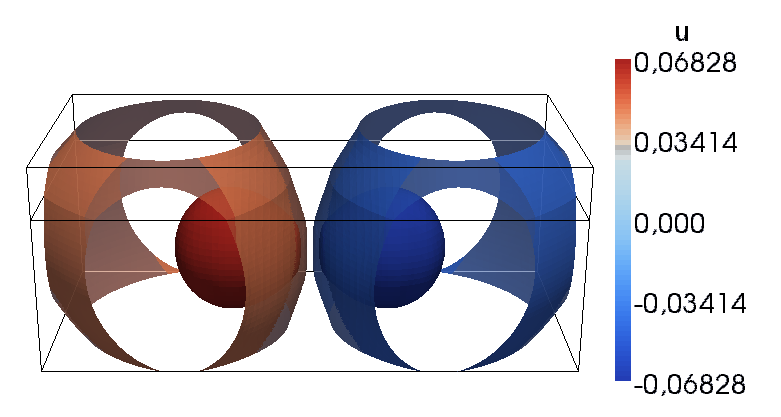
\includegraphics[width=0.8\textwidth]{fig/u_direct.png}
\caption{Solution $\boldsymbol{u}$ of the direct problem; Three isosurfaces.}
\label{u_solution}
\end{figure}

\subsection{Inverse Problem}\label{sec:exampleinvpro}
%
Here we solve the corresponding inverse problem and emphasize the effect of $\alpha$. Firstly, we have to choose the measuring grid points. For the sake of simplicity we measure $\boldsymbol{u}|_{\Gamma_h}$ on two planes
%
\begin{equation*}
	\Gamma_h:=\{(x,y,z)\in\mathbb{R}^3:0\le x\le 20,\;0\le y\le 10,\;z=1\;\text{or}\;z=1.5\},
\end{equation*}
%
i.e. on every grid point in these planes. These planes and the dipole can be seen in Figure \ref{planes_dipole}. Now it is easy to implement the discrete restriction operator $\boldsymbol{T}$, see \eqref{eq:syntheticdata} and cf. Listing \ref{sc:ud}.\\

\begin{figure}[h!]
	\centering
		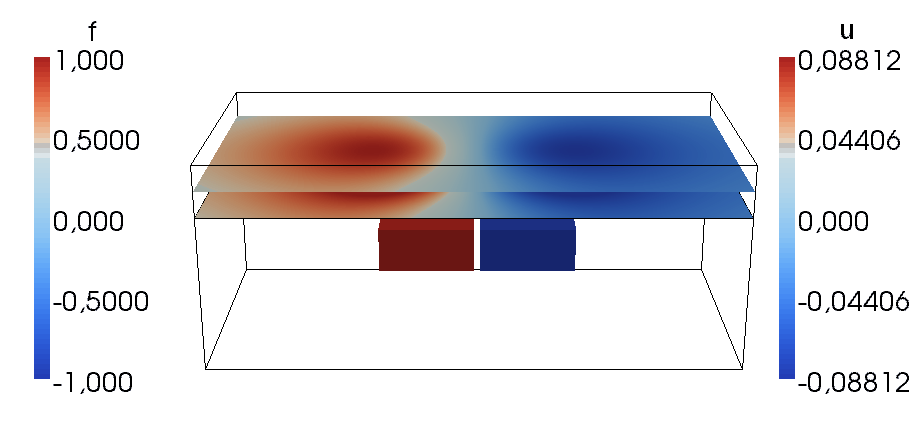
\includegraphics[width=0.8\textwidth]{fig/f_direct_and_measure_points.png}
\caption{Two planes on which the electric potential is measured and the dipole which we choose.}
\label{planes_dipole}
\end{figure}

In addition, we have to implement the penalty operator $\boldsymbol{D}$, which includes the following information. We know that the support of $f$ must be underneath the ground surface and it cannot contact the boundary. Consequently, we penalize the boundary grid points and the grid points in the air. Let $p^x_i$ be the $x$-coordinate, $p^y_i$ be the $y$-coordinate and $p^z_i$ be the $z$-coordinate of the $i$-th grid point $p$, then we chose a diagonal matrix $\boldsymbol{D}$ with corresponding matrix elements
%
\begin{equation*}
	\boldsymbol{D}_{i,i}:=\left\{\begin{array}{ll}
	1, & \text{if}\;0<p^x_i<20,\;\text{or}\;0<p^y_i<10,\;\text{or}\;-6<p^z_i<0\\
	100, & \text{else},
	\end{array}\right.
\end{equation*}
%
see \eqref{eq:damping} and cf. Listing \ref{sc:d}. Using this diagonal matrix inside the regularized term we get a good pseudo-solutions.\\

%small_alpha
\begin{figure}[h!]
	\centering
		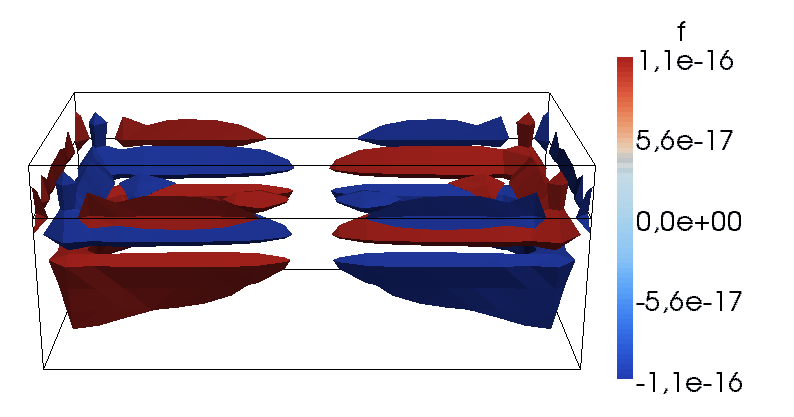
\includegraphics[width=0.8\textwidth]{fig/f_inverse_small_alpha.png}
\caption{Pseudo-solution $\boldsymbol{f}_\alpha$ for $\alpha$ which is too small.}
\label{small_alpha}
\end{figure}
%
Recalling we are searching for an optimal $\alpha$, which is large enough to apply CG method and small enough to save the relation to the true solution. To show the influence of the regularization parameter $\alpha$ to the pseudo-solution we are going to reconstruct the source $\boldsymbol{f}$ for three different $\alpha$. In the first case we set $\alpha_1=10^{-6}\cdot\max_{i=1,\ldots,n}|\boldsymbol{\Lambda}_{i,i}|$, so that the inverse cannot be computed. The result can be seen in Figure \ref{small_alpha}. The second case shows a well fitted regularization parameter $\alpha_2=0.1\cdot\max_{i=1,\ldots,n}|\boldsymbol{\Lambda}_{i,i}|$, see Figure \ref{good_alpha} and cf. Listing \ref{sc:alpha}, and in the third case $\alpha_3=1.000\cdot\max_{i=1,\ldots,n}|\boldsymbol{\Lambda}_{i,i}|$ regularized the pseudo-solution too strong, so that $\boldsymbol{f}_\alpha$ is approximately zero almost everywhere, as seen in Figure \ref{big_alpha}.\\
Note that if the $L$-curve criterion would be applied to determine the optimal $\alpha$, one has to compute the pseudo-solution $\boldsymbol{f}_\alpha$ for several $\alpha$. Subsequently, this heuristic parameter choise rule determines the best of all these solutions. That's why finding an optimal $\alpha$ by the $L$-curve criterion is expensive, but comfortable.


%good_alpha
\begin{figure}[h!]
	\centering
		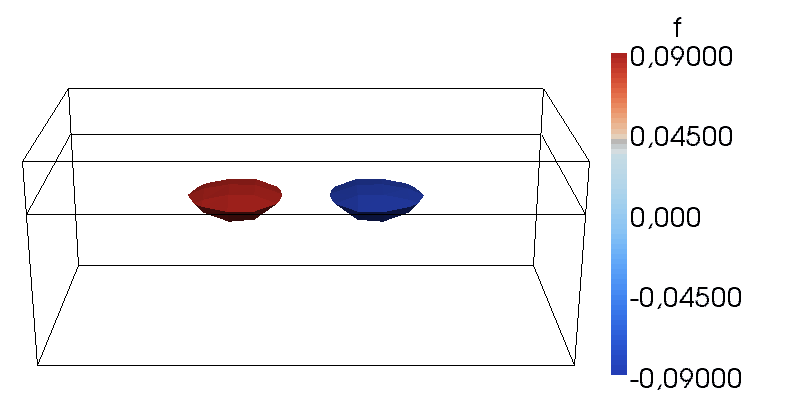
\includegraphics[width=0.8\textwidth]{fig/f_inverse_good_alpha.png}
\caption{Pseudo-Solution $\boldsymbol{f}_\alpha$ for $\alpha$ which fits the scenario.}
\label{good_alpha}
\end{figure}

%big_alpha
\begin{figure}[h!]
	\centering
		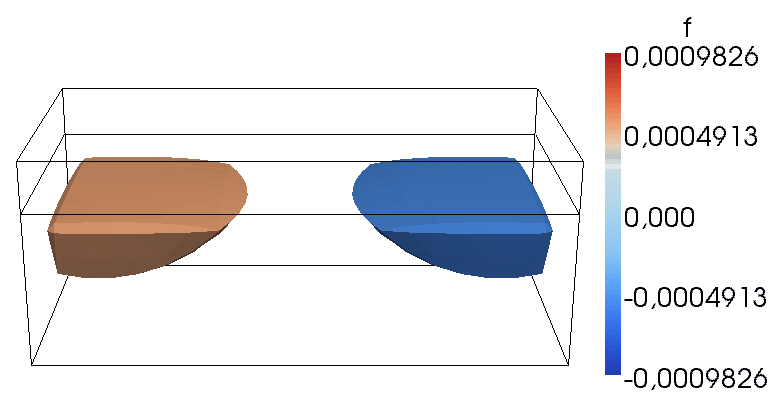
\includegraphics[width=0.8\textwidth]{fig/f_inverse_big_alpha.png}
\caption{Pseudo-Solution $\boldsymbol{f}_\alpha$ for $\alpha$ which is too large.}
\label{big_alpha}
\end{figure}


\newpage
\appendix

%\bibliography{tutorials_bib}
\bibliographystyle{plain}

\begin{thebibliography}{99}
\bibitem{bib:bra03}
D.\,Braess: \emph{Finite Elemente}, Theorie, schnelle L\"oser und Anwendungen in der Elastizit\"atstheorie, Springer-Verlag, 2003.

\bibitem{bib:gil01}
D.Gilbarg, N.S.Trudinger: Elliptic Partial Differential Equations of Second order, Second Edition, Springer-Verlag, Berlin, 2001

\bibitem{bib:had15}
J.Hadamard, Four lectures on mathematics, Columbia University Press, New York, 1915.

\bibitem{bib:kir96}
A.\,Kirsch: \textit{An Introduction to the Mathematical Theory of Inverse Problems}, Springer-Verlag, 1996.

\bibitem{bib:rie03}
A.\,Rieder: \textit{Keine Probleme mit Inversen Problemen} Eine Einf\"uhrung in ihre stabile L\"osung, Vieweg Verlag, 2003

\bibitem{bib:sal08}
S.Salsa: Partial Differential Equations in Action, From Modelling to Theory, Springer, 2008

\bibitem{bib:som12}
A.Sommer: Passive Airborne Oil Exploration - Theorie und Numerik eines linearen inversen Problems, KIT, Diploma Theses, 2012.

\bibitem{bib:tik63}
A.N.Tikhonov, Solution of incorrectly formulated problems and the regularization method, Soviet Mathematics Doklady 4(1963), 1035-1038
\end{thebibliography}

\end{document}
